\chapter{Optimierung}
Im folgenden Abschnitt soll die mathematische Modellierung der Sozialen Hierarchie, der Beutesuche, deren Einkreisen und der Angriff vorgestellt werden.


\section{Soziale Hierarchie}
Für die Optimierung wird davon ausgegangen, dass Alpha-, Beta- und Deltawolf besten Kenntnisse über den Standort der Beute haben und sich das Rudel anhand deren Positionen ausrichtet. Dazu werden pro Runde die besten drei Lösungen ermittelt und entsprechend als Alpha, Beta und Delta klassifiziert. Alle übrigen Lösungen werden zu den Omegas gezählt und damit nicht weiter untergliedert. \\
Alpha, Beta und Delta führen die Jagd (Optimierung) an und alle übrigen Omegas folgen diesen. Pro Runde werden für jeden Wolf neue Positionen anhand der Positionen von Alpha, Beta und Delta berechnet und damit die Position Wölfe immer in eine bestimmte Richtung konvergiert. Durch die Anwendung von Limits kann das Rudel wieder zusammen gezogen werden, wenn sich die einzelnen Mitglieder zu weit verstreuen, \cite[vgl. Mirjalili 2014, S.5]{MIRJALILI201446}

\section{Beutetier einkreisen}
Das Umkreisen der Beute wird mit folgenden Formeln beschrieben:
\begin{equation}
    \vec{D} = |\vec{C} \cdot \vec{X_p}(t) - \vec{X}(t) |
    \label{calcD}
\end{equation}
\begin{equation}
    \vec{X}(t+1) = \vec{X_p}(t) - \vec{A} \cdot \vec{D}
    \label{calcNextP}
\end{equation}

Wobei $t$ die momentane Iteration angibt und $\vec{A}$ und $\vec{C}$ Koeffizientenvekoren sind, $\vec{X_p}$ die Position der Beute (Prey) und $\vec{X}$ die Position eines Wolfes.\\
Der Vektor $\vec{D}$ (\autoref{calcD}) gibt die Richtung an, in die der Rest des Rudels konvergieren soll und wird zur Bestimmung des nächsten Positionsvektors eines Wolfes ($\vec{X}(t+1)$, \autoref{calcNextP}) gebraucht.\\
Die Vektoren $\vec{A}$ und $\vec{C}$ werden mit folgenden Formeln bestimmt:

\begin{equation}
    \vec{A} = 2 \vec{a} \cdot \vec{r_1} - \vec{a}
    \label{calcA}
\end{equation}
\begin{equation}
    \vec{C} = 2 \vec{r_2}
    \label{calcC}
\end{equation}

Die Komponenten von $\vec{a}$ werden mit jeder Iteration linear von $2$ bis $0$ verringert und $\vec{r_1}$ und $\vec{r_2}$ sind Zufallsvektoren in $[0,1]$.\\
\begin{figure}[ht]
    \begin{center}
        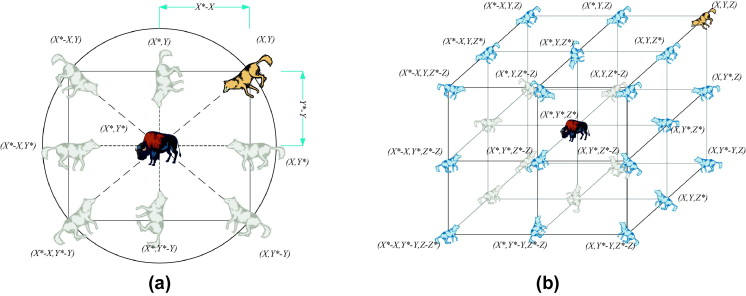
\includegraphics[width=0.7\textwidth]{assets/img/Updating_position_of_gray_wolves_in_GWO.jpg}
        \caption[Positionsneuberechnung im GWO]{Positionsneuberechnung im GWO \cite{MIRJALILI201446}}
        \label{gwo_newPos}
    \end{center}
\end{figure}

In \autoref{gwo_newPos} wird dargestellt, welchen Effekt \autoref{calcD} und \autoref{calcNextP} haben. In \autoref{gwo_newPos} (a) wird dargestellt, wie ein Wolf mit Position (X, Y) seine Position hin zur Beute auf Position (X*, Y*) verändern kann. Durch Variieren der Vektoren $\vec{A}$ und $\vec{C}$ können verschiedene Positionen rund um den Alpha eingenommen werden. \\
Durch die Vektoren $\vec{r_1}$ und $\vec{r_2}$ kann ein Wolf jede zufällige Position rund um die Beute, wie in \autoref{gwo_newPos} dargestellt, erreichen, (\cite[vgl. Mirjalili 2014, S.6]{MIRJALILI201446}).

\section{Jagd}
Um das Jagdverhalten zu simulieren, wird angenommen, dass Alpha, Beta und Delta das beste Wissen über die Beute haben. Dazu werden bei jeder Iteration die Wölfe neu klassifiziert und die drei besten Lösungen als Alpha, Beta und Delta klassifiziert. Die übrigen Rudelmitglieder konvergieren bei der Neuberechnung ihrer Positionen in Richtung dieser besten Lösungen. Somit wird der Schwarm mit jeder Iteration hin zu besten bisherigen Lösung gezogen. \\
Dies wird mit folgenden Formeln bestimmt:

\begin{equation}
    \vec{D_\alpha} = |\vec{C_1} \cdot \vec{X_\alpha} - \vec{X}|;
    \vec{D_\beta} = |\vec{C_2} \cdot \vec{X_\beta} - \vec{X}|;
    \vec{D_\delta} = |\vec{C_3} \cdot \vec{X_\delta} - \vec{X}|
    \label{calcD_abc}
\end{equation}

\begin{equation}
    \vec{X_1} = \vec{X_\alpha} - \vec{A_1} \cdot (\vec{D_\alpha});
    \vec{X_2} = \vec{X_\beta} - \vec{A_2} \cdot (\vec{D_\beta});
    \vec{X_3} = \vec{X_\delta} - \vec{A_3} \cdot (\vec{D_\delta});
    \label{calcX_123}
\end{equation}

\begin{equation}
    \vec{X}(t+1) = \frac{\vec{X_1} + \vec{X_2} + \vec{X_3}}{3}
    \label{calcNextP2}
\end{equation}

Hier ist deutlich der Einfluss von Alpha, Beta und Delta auf die neue Position des einzelnen Wolfes zu sehen, der den Schwarm in Richtung der Beute konvergieren lässt, siehe \autoref{gwo_vectorizing}, (\cite[vgl. Mirjalili 2014, S.7]{MIRJALILI201446}).

\begin{figure}[ht]
    \begin{center}
        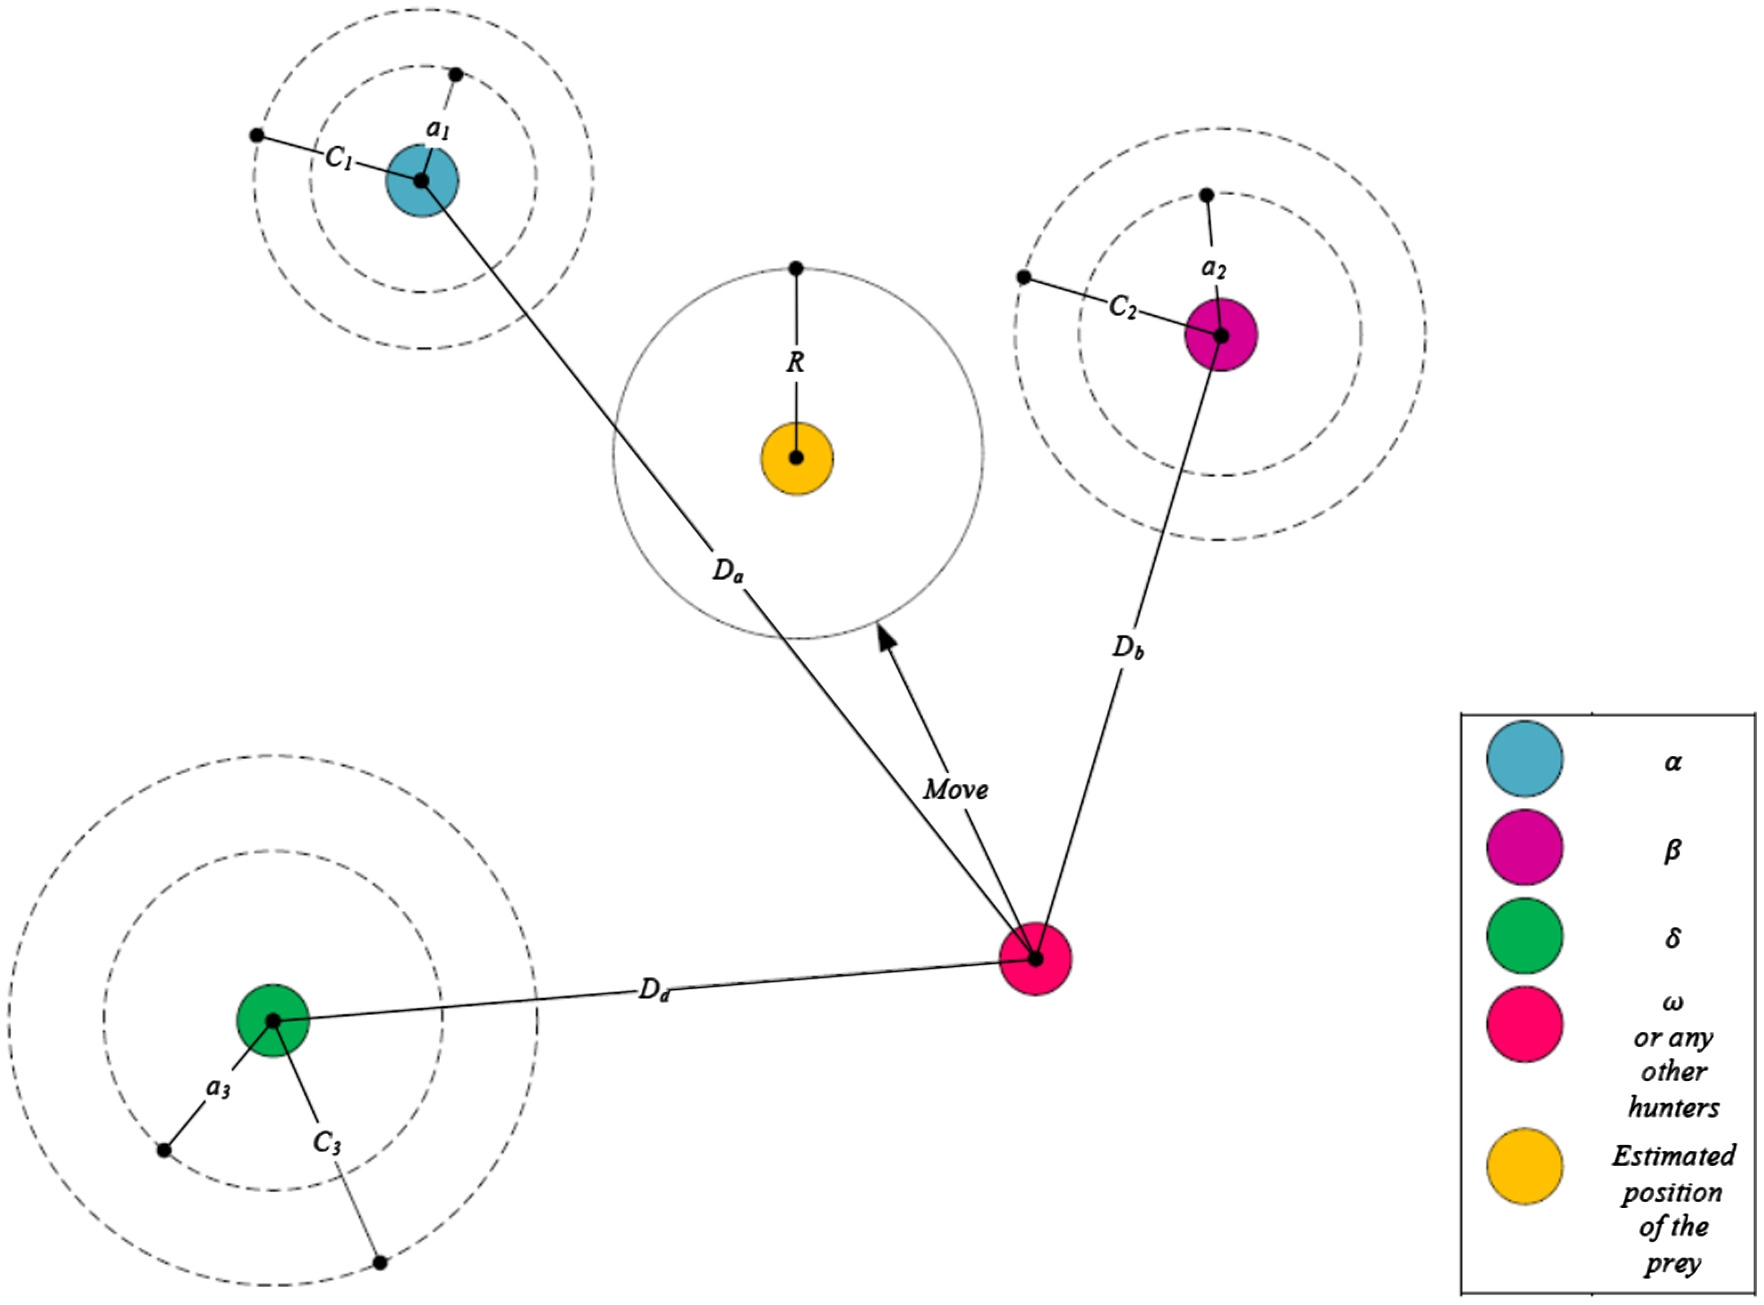
\includegraphics[width=1.0\textwidth]{assets/img/tgis12517-fig-0002-m.png}
        \caption[Positionsneuberechnung im GWO]{Positionsneuberechnung im GWO \cite{MIRJALILI201446}}
        \label{gwo_vectorizing}
    \end{center}
\end{figure}

\section{Beute angreifen}
Für das Angreifen der Beute wird kein extra Schritt und auch keine weitere Formel benötigt, sondern es geschieht mittels der Verringerung des Vektors $\vec{a}$ und damit auch des Vektors $\vec{A}$, der im Interval $[-a, a]$ liegt. Mit $\vec{A}$ in $[-1, 1]$ kann die nächste Position eines Wolfes immer auf jeder Position zwischen seiner jetzigen Position und der Position der Beute sein. \\
Somit attackiert gezwungenermaßen jeder Wolf für $|A| < 1$ die Beute und die einzelnen Wölfe konzentrieren sich auf einen Punkt, dem gesuchten Optimum, (\cite[vgl. Mirjalili 2014, S.8]{MIRJALILI201446}). 
\section{Pseudocode}
Folgend der Pseudocode des GWO:
\begin{figure}[ht]
    \begin{center}
        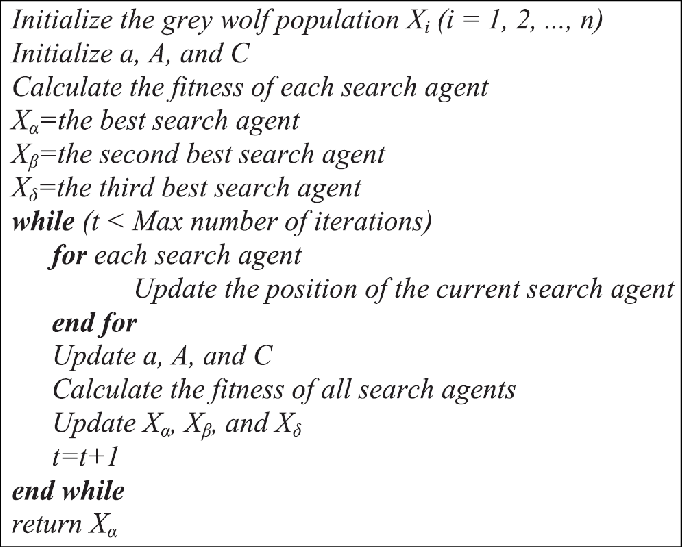
\includegraphics[width=0.7\textwidth]{assets/img/Pseudo-code-of-Grey-Wolf-Optimization-GWO-algorithm.png}
        \caption[Pseudocode GWO]{Pseudocode GWO \cite{MIRJALILI201446}}
        \label{gwo_pseudocode}
    \end{center}
\end{figure}